\documentclass[10pt]{standalone}
\usepackage{tikz}
\usetikzlibrary{shapes.geometric,calc,decorations.pathreplacing}

\tikzset{
    file/.style = {
        draw, fill=blue!20, rectangle, align=center,
        outer sep=0,
        inner sep=0,
        minimum width={width("Queue")+2pt},
        minimum height={3cm},
        font=\normalsize
    },
    unit/.style = {
        draw, fill=gray!20, rectangle, align=center,
        outer sep=0,
        inner sep=0,
        minimum width={width("FALU2")+2pt},
        minimum height={2cm},
        font=\normalsize
    },
    anno/.style = {
        rectangle, align=center,
        outer sep=0,
        inner sep=0,
        minimum height={2cm},
        font=\scriptsize
    },
    dot/.style = {
        circle,fill=#1,inner sep=0,minimum size=4pt
    }
}

\expandafter\def\csname FixQ \endcsname{Fix\\ Issue\\ Queue}
\expandafter\def\csname FixF \endcsname{Fix\\ Reg\\ File}
\expandafter\def\csname FltQ \endcsname{Float\\ Issue\\ Queue}
\expandafter\def\csname FltF \endcsname{Float\\ Reg\\ File}
\newcommand{\FU}[1]{\node[unit](#1){#1};}
\newcommand{\QF}[2]{\node[file](#1#2){\csname #1 \endcsname};}

\newcommand{\xy}[1]{\coordinate (#1);}
\newcommand{\cell}[1]{\node[text width=#1cm]{};}

\begin{document}
\thispagestyle{empty}

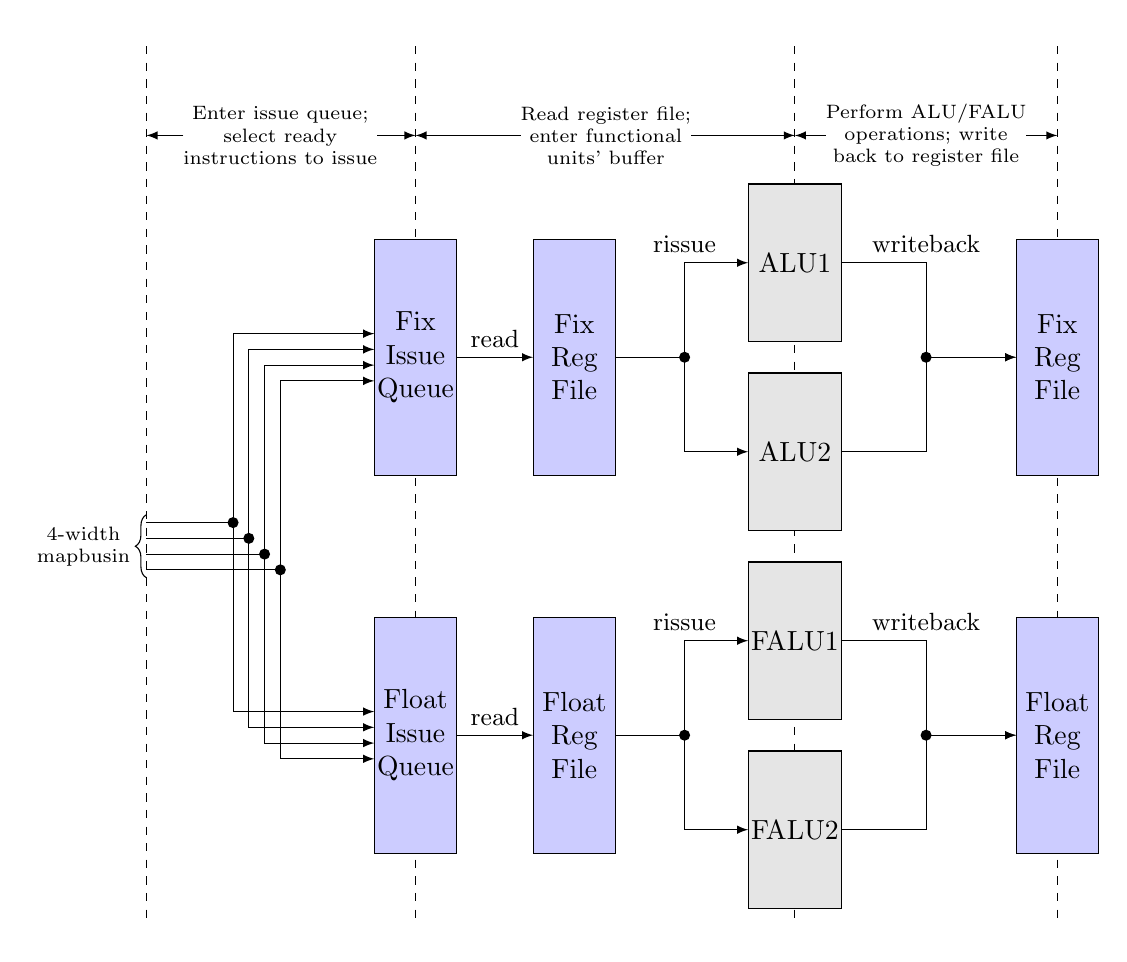
\begin{tikzpicture}

% 1. matrix layout
\node[matrix,very thin,column sep=1.4cm,row sep=1.2cm] (matrix) at (0,0) {
  \xy{u1} &         & \xy{u2}    &            &         & \xy{u3}    & \cell{.3} & \xy{u4} \\
          & \xy{a0} & \cell{1}   & \xy{a1}    &         &            & \xy{a2}   & \\
          &         &            &            &         & \xy{ALU1}  &           & \\
          &         & \xy{FixQ1} & \xy{FixF1} & \xy{n1} &            & \xy{n3}   & \xy{FixF2} \\
          &         &            &            &         & \xy{ALU2}  &           & \\
  \xy{m1} & \xy{m2} &            &            &         &            &           & \\
          &         &            &            &         & \xy{FALU1} &           & \\
          &         & \xy{FltQ1} & \xy{FltF1} & \xy{n2} &            & \xy{n4}   & \xy{FltF2} \\
          &         &            &            &         & \xy{FALU2} &           & \\
  \xy{b1} &         & \xy{b2}    &            &         & \xy{b3}    &           & \xy{b4} \\
};

% 2. vertical lines
\draw [dashed] 
  (u1) -- (b1) (u2) -- (b2) (u3) -- (b3) (u4) -- (b4);

% 3. align block boxes -- use \foreach later
\node[file] (FixQ1) at (FixQ1) {Fix\\ Issue\\ Queue};
\node[file] (FltQ1) at (FltQ1) {Float\\ Issue\\ Queue};
\node[file] (FixF1) at (FixF1) {Fix\\ Reg\\ File};
\node[file] (FltF1) at (FltF1) {Float\\ Reg\\ File};
\node[file] (FixF2) at (FixF2) {Fix\\ Reg\\ File};
\node[file] (FltF2) at (FltF2) {Float\\ Reg\\ File};
\node[unit] (ALU1)  at (ALU1)  {ALU1};
\node[unit] (ALU2)  at (ALU2)  {ALU2};
\node[unit] (FALU1) at (FALU1) {FALU1};
\node[unit] (FALU2) at (FALU2) {FALU2};

% 4. arrows and label
\draw[-latex,font=\small] (FixQ1) -- (FixF1) node[midway,above] {read};
\draw[-latex,font=\small] (FltQ1) -- (FltF1) node[midway,above] {read};
\draw[-latex,font=\small] (FixF1) -- (n1) |- (ALU1) node[midway,above] {rissue};
\draw[-latex,font=\small] (FixF1) -- (n1) |- (ALU2);
\draw[-latex,font=\small] (FltF1) -- (n2) |- (FALU1) node[midway,above] {rissue};
\draw[-latex,font=\small] (FltF1) -- (n2) |- (FALU2);
\draw[-latex,font=\small] (ALU1)  -| (n3) node[midway,above] {writeback} -- (FixF2);
\draw[-latex,font=\small] (ALU2)  -| (n3) -- (FixF2);
\draw[-latex,font=\small] (FALU1) -| (n4) node[midway,above] {writeback} -- (FltF2);
\draw[-latex,font=\small] (FALU2) -| (n4) -- (FltF2);

\draw[-latex] ($(m1)+(0, .3)$) -- ($(m2)+(-.3, .3)$) |- ($(FixQ1.west)+(0, .3)$);
\draw[-latex] ($(m1)+(0, .1)$) -- ($(m2)+(-.1, .1)$) |- ($(FixQ1.west)+(0, .1)$);
\draw[-latex] ($(m1)+(0,-.1)$) -- ($(m2)+( .1,-.1)$) |- ($(FixQ1.west)+(0,-.1)$);
\draw[-latex] ($(m1)+(0,-.3)$) -- ($(m2)+( .3,-.3)$) |- ($(FixQ1.west)+(0,-.3)$);
\draw[-latex] ($(m1)+(0, .3)$) -- ($(m2)+(-.3, .3)$) |- ($(FltQ1.west)+(0, .3)$);
\draw[-latex] ($(m1)+(0, .1)$) -- ($(m2)+(-.1, .1)$) |- ($(FltQ1.west)+(0, .1)$);
\draw[-latex] ($(m1)+(0,-.1)$) -- ($(m2)+( .1,-.1)$) |- ($(FltQ1.west)+(0,-.1)$);
\draw[-latex] ($(m1)+(0,-.3)$) -- ($(m2)+( .3,-.3)$) |- ($(FltQ1.west)+(0,-.3)$);

%5. annotation
\coordinate (a0) at ($(a0)+(.3,.3)$);
\coordinate (a1) at ($(a1)+(.4,.3)$);
\coordinate (a2) at ($(a2)+(.0,.3)$);
\node[anno] (a0) at (a0) {Enter issue queue;\\ select ready\\ instructions to issue};
\node[anno] (a1) at (a1) {Read register file;\\ enter functional\\ units' buffer};
\node[anno] (a2) at (a2) {Perform ALU/FALU\\ operations; write\\ back to register file};

\draw[-latex] (a0) -- (a0-|u1);
\draw[-latex] (a0) -- (a0-|u2);
\draw[-latex] (a1) -- (a1-|u2);
\draw[-latex] (a1) -- (a1-|u3);
\draw[-latex] (a2) -- (a1-|u3);
\draw[-latex] (a2) -- (a1-|u4);

%6. curly brace: 4-width mapbusin
\draw [decorate,decoration={brace,amplitude=4pt},xshift=-2pt,yshift=0pt]
  ($(m1)+(0,-.4)$) -- ($(m1)+(0, .4)$)
  node [xshift=-.8cm,midway,align=center,font=\scriptsize]{4-width\\ mapbusin};

%7. add dots at inter-connection points
\node[dot=black] at ($(m2)+(-.3, .3)$) {};
\node[dot=black] at ($(m2)+(-.1, .1)$) {};
\node[dot=black] at ($(m2)+( .1,-.1)$) {};
\node[dot=black] at ($(m2)+( .3,-.3)$) {};
\node[dot=black] at (n1) {};
\node[dot=black] at (n2) {};
\node[dot=black] at (n3) {};
\node[dot=black] at (n4) {};


\end{tikzpicture}
\end{document}

